\chapter{Architektura oraz założenia systemu}
Przed faktycznym rozpoczęciem prac nad złożonym systemem programowym należy najpierw zastanowić się nad jego architekturą.
Ułatwia to określenie wymagań, celów, a także potencjalnych trudności które można napotkać w trakcie prac. 

\section{Rodzaje systemów rysujących}
Głównym założeniem projektu jest stworzenie uniwersalnego, modularnego systemu rysującego.
Systemy tego typu przyjmują najczęściej formę, którą można określić jako punkt między dwoma ekstremami. 

\subsection{Moduł niezależny}
\label{Subsection_module_types_engine}
Po jednej stronie spektrum znajduje się system prawie całkowicie niezależny. Swoim działaniem jest zbliżony do silników do gier, gdzie skrypt klienta zostaje periodycznie wywołany w celu zmiany wewnętrznego stanu modułu. System jest w takim przypadku odpowiedzialny za większość kontroli przepływu programu, w tym operacji związanych z rysowaniem, inicjalizację okna, ruch kamery w odpowiedzi na interakcje z użytkownikiem, generowanie modelu 3D na podstawie pliku wejściowego, czy obliczanie zaawansowanych efektów świetlnych. Silnik przechowuje listę obiektów sceny wraz z ich parametrami, takimi jak translacja, materiał czy wzajemne relacje, które wykorzystuje do renderowania obrazu. 

Zastosowanie takiej metody zwiększa potencjał wydajnościowy silnika oraz wyraźnie zmniejsza nakład pracy dla programisty piszącego aplikację kliencką. Pozwala to także na potencjalną całkowitą niezależność od użytego API graficznego oraz systemu operacyjnego, gdyż możliwa jest realizacja w formie interfejsu, której implementacje odpowiadać będą poszczególnym konfiguracjom. Dużą wadą jest jednak konieczność zmiany kodu i rekompilacji modułu w przypadku potrzeby dodania nowej funkcjonalności lub zmiany sposobu działania już istniejącej. 

Uproszczona wizualizacja przykładowej wymiany operacji systemu tego typu została przedstawiona na rys. \ref{UML_Sequence_Module_Engine}. Widoczne jest na nim przeniesienie większości operacji na moduł silnika, który steruje działaniem programu.

\begin{figure}[ht!]
	\centering
	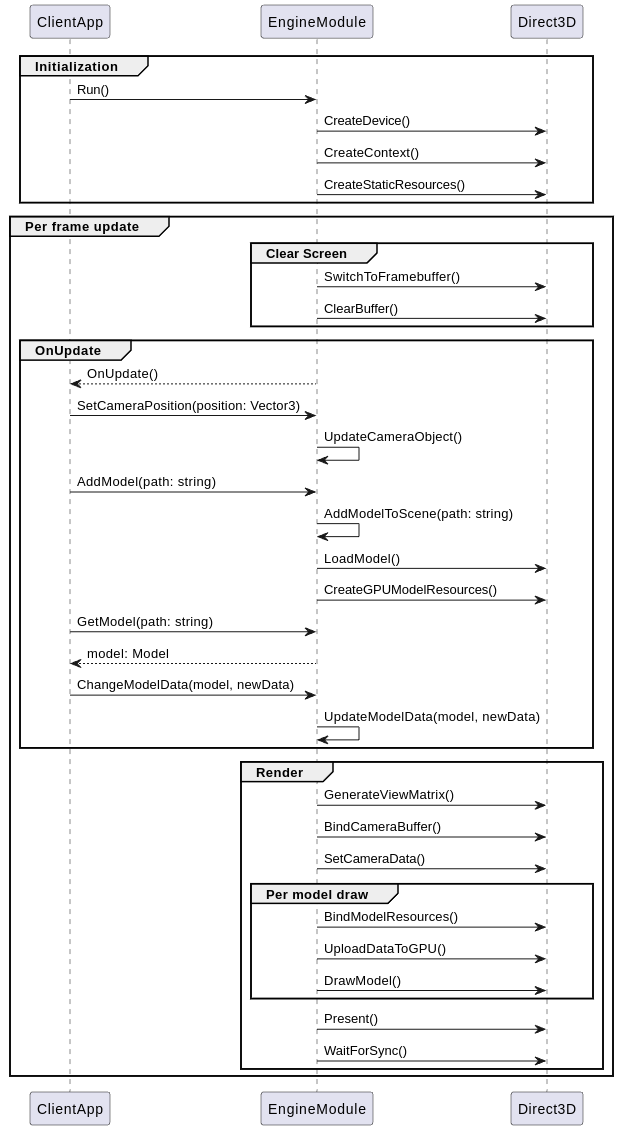
\includegraphics[width=300px]{uml/module_type_engine.png}
	\caption{Diagram przedstawiający sekwencję operowania modułu typu niezależnego z aplikacją klienta.}
	\label{UML_Sequence_Module_Engine}
\end{figure}

\vfill
\clearpage

\subsection{Abstrakcja nad API}
\label{Subsection_module_types_abstraction}
Przeciwieństwem jest moduł będący abstrakcją nad niskopoziomowymi API graficznymi. Udostępnia on uniwersalne API niezależne od systemu operacyjnego oraz końcowego API graficznego, nie zabierając przy tym kontroli nad procesem renderowania. Aplikacja klienta zarządza przepływem programu, przechowywaniem i wyświetlaniem obiektów oraz ich parametrami, a także nad dokładnym rozkładem czasowym oraz kolejnością wywoływanych metod. Ogranicza to złożoność modułu, który przejmuje na siebie utworzenie bardziej przystępnego dla programistów interfejsu.

Oczywistą wadą takiego rozwiązania jest zwiększony nakład pracy dla programisty aplikacji klienta. Ze względu na asynchroniczną charakterystykę współczesnych układów graficznych oraz ich złożoność ograniczony może zostać także potencjał wydajnościowy końcowej aplikacji. W zamian oddana jest możliwość dowolnego rozszerzania funkcjonalności modułu bez konieczności znania i modyfikacji jego kodu źródłowego.

Analogiczna do rys. \ref{UML_Sequence_Module_Engine} wizualizacja dla wersji abstrakcji została pokazana na rys. \ref{UML_Sequence_Module_Abstraction}.

\begin{figure}[ht!]
	\centering
	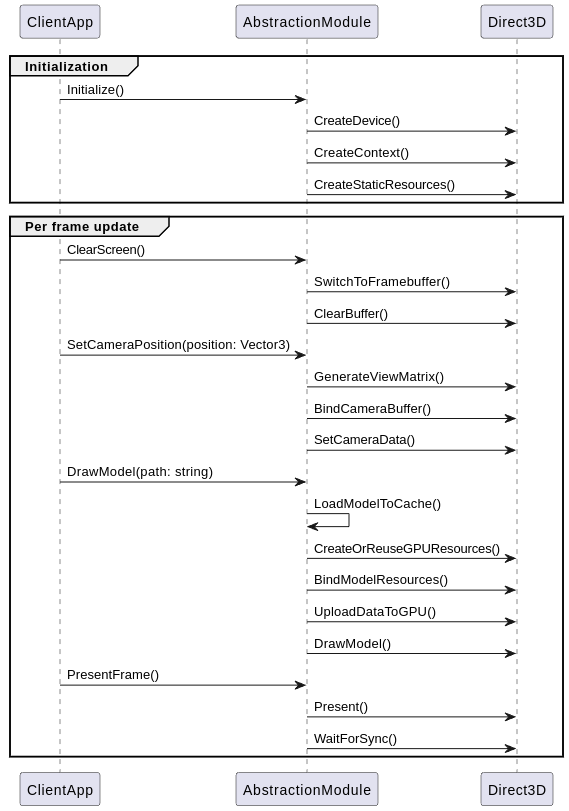
\includegraphics[width=250px]{uml/module_type_abstraction.png}
	\caption{Diagram przedstawiający sposób działania modułu abstrakcji.}
	\label{UML_Sequence_Module_Abstraction}
\end{figure}

\section{Przyjęte założenia projektowe}
Projektowany system przyjmuje formę hybrydową, korzystającą z zalet obu przedstawionych podejść do projektowania tego typu systemu. 

Głównym założeniem i podstawą implementacji zostanie utworzenie systemu warstwowego, pozwalającego na korzystanie z modułu jako abstrakcji nad API Direct3D 11 w warstwach niższych, a także na pracę w trybie niezależnym przy wyższych poziomach abstrakcji, które same będą korzystać z niższych elementów do swojego działania. Każdy z etapów umożliwiać będzie także dostęp do podległych mu komponentów. Takie podejście umożliwia mieszanie ze sobą różnych paradygmatów nie ograniczając ani potencjalnej funkcjonalności, ani przystępności dla nowych projektów i programistów.

Logistycznie projekt został podzielony na następujące warstwy:

\subsection{\textbf{Core} - Warstwa rdzeniowa}
Klasyczna warstwa abstrakcji. Grupuje często używane funkcje oraz struktury z DirectX do łatwych w użyciu elementów obiektowych, takich jak Window, Shader, Framebuffer, czy Mesh. Udostępnia funkcjonalność wczytywania z dysku plików tekstur i modeli. Do zadań tej warstwy należy też zarządzenia pamięcią oraz cyklem życia obiektów, co odbywa się automatycznie stosując inteligentne wskaźniki ze standardu C++11 oraz ComPtr z bibliotek WinAPI.

Warstwa ta udostępnia interfejs zbliżony konceptem do modułu abstrakcji z sekcji \ref{Subsection_module_types_abstraction}. 

\subsection{\textbf{Scene} - Warstwa sceny}
Na tym poziomie znajdują się wysokopoziomowe struktury oraz metody wczytywania i zarządzania sceną oraz jej komponentami. Automatyzowane jest tutaj między innymi wczytywanie z pliku pełnego modelu wraz z jego teksturami i parametrami materiałów. Segment ten odpowiada też za zachowanie wzajemnych relacji między obiektami z uwzględnieniem ich transformacji.

\subsection{\textbf{Engine} - Warstwa renderująca}
Implementacja modułu typu niezależnego. Aplikacja klienta przekazuje przy inicjalizacji parametry sceny, pozycje oraz ustawienia modeli, wirtualnej kamery i oświetlenia. Wartości te mogą być modyfikowane w przekazanej do modułu funkcji typu callback, wywoływanej automatycznie przed rysowaniem kolejnej klatki obrazu, tak jak zostało to opisane w sekcji \ref{Subsection_module_types_engine}. Możliwe jest także przełączenie w tryb ręczny zbliżony do wersji z podrozdziału \ref{Subsection_module_types_abstraction}, w którym za wywoływanie funkcji rysowania oraz synchronizację odpowiedzialna jest aplikacja klienta. Na tym poziomie obecna jest także logika ułatwiająca pracę z buforami, oświetleniem, pakiet standardowych shader'ów czy menadżer zasobów.

Interakcja między aplikacją klienta, a modułem została przedstawiona na rys. \ref{UML_Sequence_Module_Final}. W przypadku trybu ręcznego etap \textit{EngineLoop} zostaje pominięty i jego funkcjonalność przejmuje aplikacja klienta.

\begin{figure}[ht!]
	\centering
	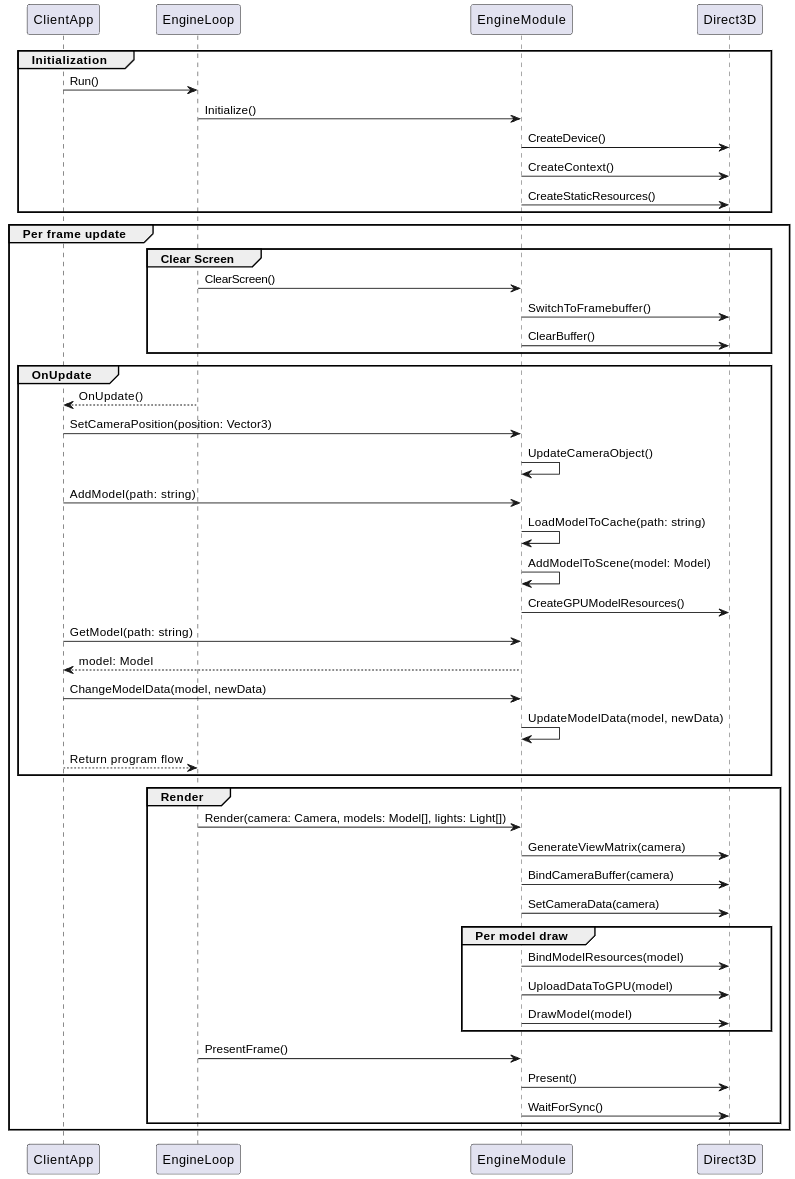
\includegraphics[width=350px]{uml/module_type_final.png}
	\caption{Diagram przedstawiający sposób działania modułu abstrakcji.}
	\label{UML_Sequence_Module_Final}
\end{figure}